\begin{tikzpicture}
    \begin{axis}[
    ybar,
    width=\linewidth, height=5cm,
    ylabel={$t \ (\si{ms})$}, ylabel near ticks, ymin=10, ymax=100000,
    xtick={1, 2, 3}, xticklabels={$\ang{0}$, $\ang{0.0001}$, $\ang{0.01}$},
    xlabel={$\rho$}, xmin=0.5, xmax=3.5, xtick pos=left, point meta=rawy,
    nodes near coords, every node near coord/.append style={rotate=90, anchor=west,
    /pgf/number format/.cd,fixed,precision=6},
    legend style={at={(0.5,-0.35)}, anchor=north,legend columns=-1},
    bar width=7, ymode=log, log origin=infty, max space between ticks=20
    ]
        \addplot coordinates {(1, 1197.43) (2, 1349.07) (3, 6509.00)};
        \addplot coordinates {(1, 160.68) (2, 161.80) (3, 872.22)};
        \addplot coordinates {(1, 323.94) (2, 339.23) (3, 392.29)};
        \addplot coordinates {(1, 324.35) (2, 328.85) (3, 352.24)};
        \addplot coordinates {(1, 170.79) (2, 171.53) (3, 364.04)};
        \addplot coordinates {(1, 405.53) (2, 1545.45) (3, 362.30)};
        \legend{ANG, INT, SPH, PLN, PYR, COM}
    \end{axis}
\end{tikzpicture}